\documentclass{beamer}
\usepackage{amsmath}
\usepackage{graphicx}


\usepackage{listings}
\usepackage{color}

\definecolor{dkgreen}{rgb}{0,0.6,0}
\definecolor{gray}{rgb}{0.5,0.5,0.5}
\definecolor{mauve}{rgb}{0.58,0,0.82}

\lstset{frame=tb,
  language=Java,
  aboveskip=3mm,
  belowskip=3mm,
  showstringspaces=false,
  columns=flexible,
  basicstyle={\small\ttfamily},
  numbers=none,
  numberstyle=\tiny\color{gray},
  keywordstyle=\color{blue},
  commentstyle=\color{dkgreen},
  stringstyle=\color{mauve},
  breaklines=true,
  breakatwhitespace=true,
  tabsize=3
}




\graphicspath{ {./images/} }

\title{Least squares}
\subtitle{Sample Subtitle}
\author{Juan V. Vía}
\institute{}
\date{\today}

%\usetheme{lucid}
\begin{document}
% -------------------------------------------------------------------------
\frame[t] {
	\titlepage
}
% -------------------------------------------------------------------------
\frame[t] {
	\frametitle{Example}
	\framesubtitle{Showing why least squares}
	We have a variable $y$. We know that it's dependent of another variable $x$ in some
	way. But we don't know how, exactly.

	So we go to the field and measure certain points. Those that we can reach. Six of them.
	$$(2,5),(5,5),(7,8),(11,7),(14,9),(18,7)$$

	That is: at $x=2$ we measure $y=5$, at $x=5$ we measure $y=5$ again, but
	at $x=7$ we got $y=8$, and so on.
}
% -------------------------------------------------------------------------
\frame[t] {
	\frametitle{Example}
	\framesubtitle{Showing why least squares}
	Back to desk we plot these points.
	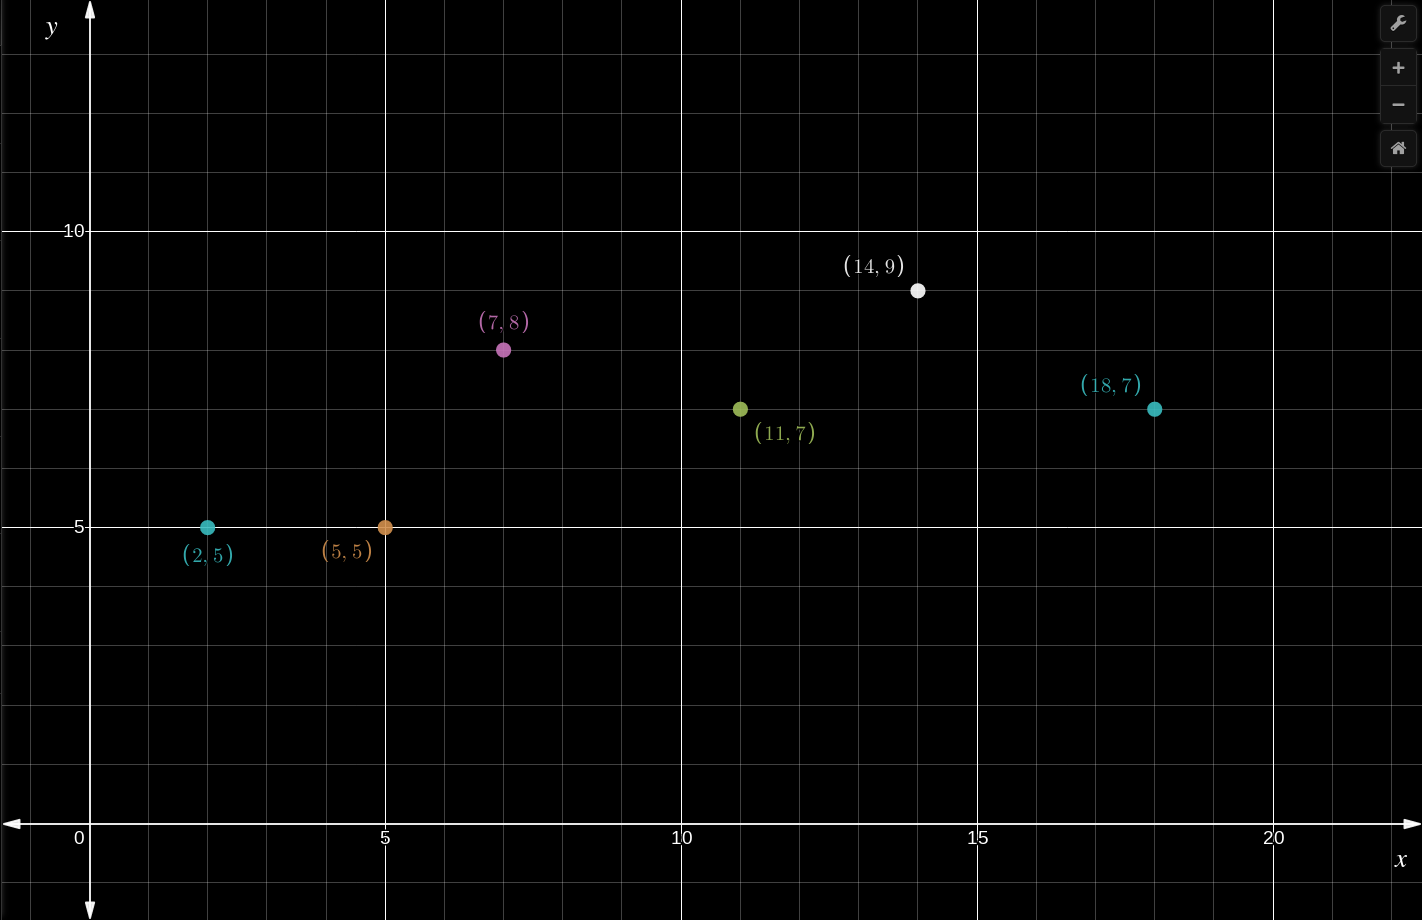
\includegraphics[width=8cm]{points}

	There is a model lurking in these points? A line perhaps?
}
% -------------------------------------------------------------------------
\frame[t] {
	\frametitle{Example}
	\framesubtitle{Showing why least squares}
	Let's start by tracing a line wich "best fit" that data

	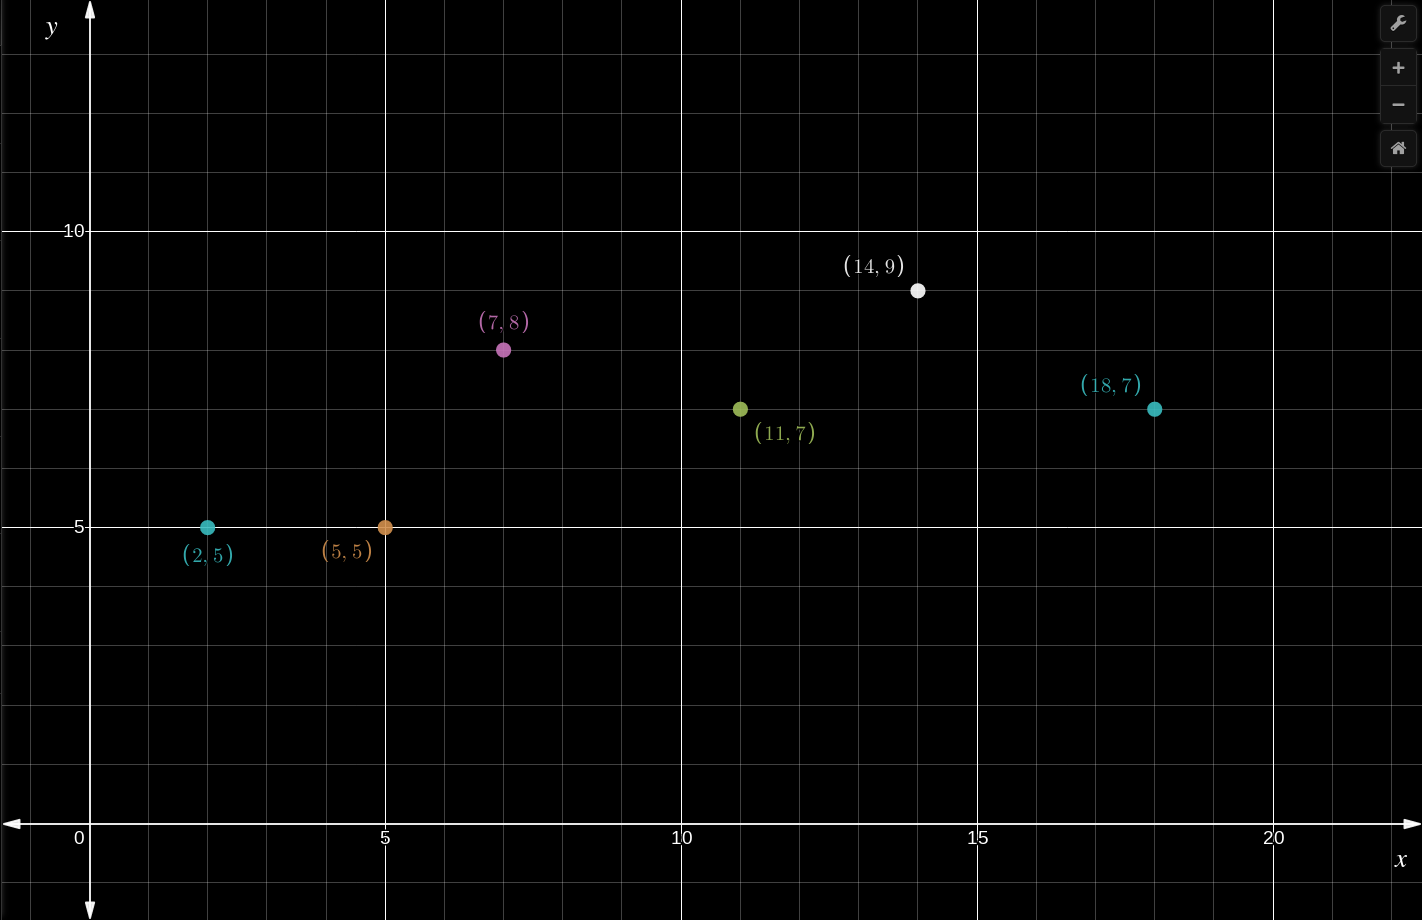
\includegraphics[width=8cm]{points}

	Why a line? To warm the modeling machine in our minds we are considering a line,
	a one degree polynomial.
}
% -------------------------------------------------------------------------
\frame[t] {
	\frametitle{Example}
	\framesubtitle{Showing why least squares}
	What line to plot? How to choose that line?

	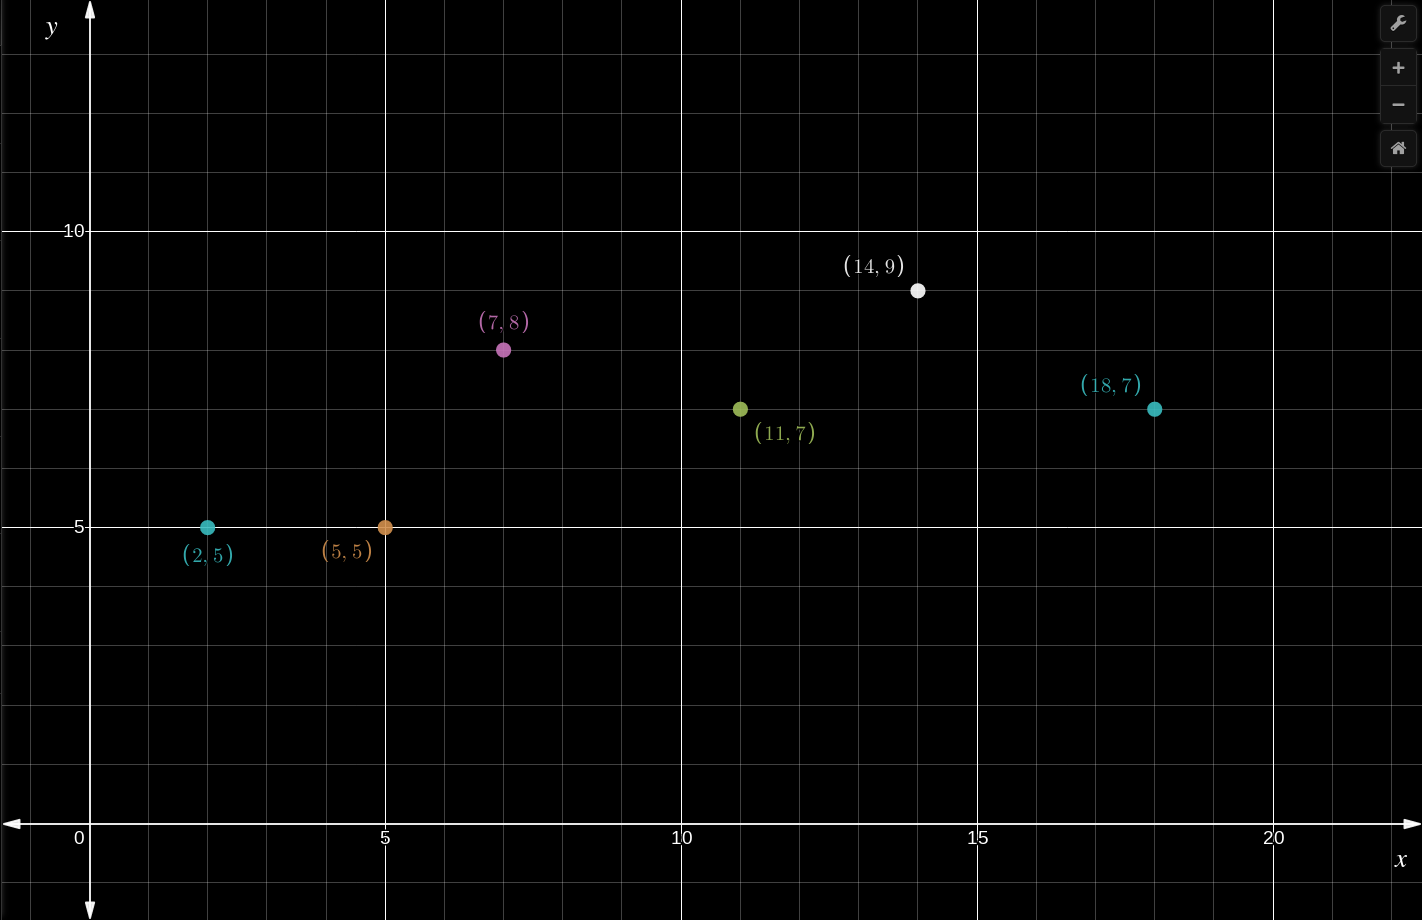
\includegraphics[width=8cm]{points}

	Enter the math...

}
% -------------------------------------------------------------------------
\frame[t] {
	\frametitle{Example}
	\framesubtitle{Showing why least squares}

	A very common way to express a line in the plane is
	% using the slope-intercept form in the cartesian plane 
	% (
	isolating
	$y$ as a polynomial function of $x$:
	% )
	$$
		y = mx + b
	$$

	From this equation we can see that $m$ is the \textit{slope} of the line and $b$ is
	the \textit{y-intercept} (the value of $y$ when $x=0$).
	\medskip

	Will be handy for us to write this equation using vector notation:
	$$y=
		\begin{bmatrix} x & 1 \end{bmatrix}
		\begin{bmatrix} m\\ b \end{bmatrix}$$

	And switching terms:
	$$\begin{bmatrix} x & 1 \end{bmatrix}
		\begin{bmatrix} m\\ b \end{bmatrix}=y$$
}
% -------------------------------------------------------------------------
\frame[t] {
	\frametitle{Example}
	\framesubtitle{Showing why least squares}

	Ok. Fine. This form
	$$\begin{bmatrix} x & 1 \end{bmatrix}
		\begin{bmatrix} m\\ b \end{bmatrix}=y$$
	will be a useful one because we know $x$ and $y$ in six points.
	For example take the first point $(2,5)$
	$$\begin{bmatrix} 2 & 1 \end{bmatrix}
		\begin{bmatrix} m\\ b \end{bmatrix}=5$$
}
% -------------------------------------------------------------------------
\frame[t] {
	\frametitle{Example}
	\framesubtitle{Showing why least squares}

	And yes, your guess is true. We can incorporate the second point $(5,5)$ and get
	$$\begin{bmatrix} 2 & 1 \\
                5 & 1\end{bmatrix}
		\begin{bmatrix} m\\ b \end{bmatrix}=\begin{bmatrix} 5\\ 5 \end{bmatrix}$$

	Doing the product you can workout $m$ and $b$ from this equation. $m=0$ and $b=5$.
	Because the matrix is square. And invertible by the way.

}
% -------------------------------------------------------------------------
\frame[t] {
	\frametitle{Example}
	\framesubtitle{Showing why least squares}

	Going further, incorporate the third point.
	$$
		\begin{bmatrix} 2 & 1 \\
                5 & 1 \\
                7 & 1\end{bmatrix}
		\begin{bmatrix} m\\ b \end{bmatrix}=\begin{bmatrix} 5\\ 5 \\ 8 \end{bmatrix}
	$$
	This invalidate the previous result. $m$ cannot be $0$ more. Neither $b$ with $5$.

	Actually, henceforth the equation is over-determined and have no solution.

}
% -------------------------------------------------------------------------
\frame[t] {
	\frametitle{Example}
	\framesubtitle{Showing why least squares}

	Fourth point.
	$$
		\begin{bmatrix} 2  & 1 \\
                5  & 1 \\
                7  & 1 \\
                11 & 1\end{bmatrix}
		\begin{bmatrix} m\\ b \end{bmatrix}=\begin{bmatrix} 5\\ 5 \\ 8 \\ 7\end{bmatrix}
	$$

}
% -------------------------------------------------------------------------
\frame[t] {
	\frametitle{Example}
	\framesubtitle{Showing why least squares}

	Fifth point.
	$$
		\begin{bmatrix} 2  & 1 \\
                5  & 1 \\
                7  & 1 \\
                11 & 1 \\
                14 & 1\end{bmatrix}
		\begin{bmatrix} m\\ b \end{bmatrix}=\begin{bmatrix} 5\\ 5 \\ 8 \\ 7 \\ 9\end{bmatrix}
	$$

}
% -------------------------------------------------------------------------
\frame[t] {
	\frametitle{Example}
	\framesubtitle{Showing why least squares}
	Sixth and last point.
	$$\begin{bmatrix} 2  & 1 \\
                5  & 1 \\
                7  & 1 \\
                11 & 1 \\
                14 & 1 \\
                18 & 1
		\end{bmatrix}
		\begin{bmatrix} m\\ b \end{bmatrix}=\begin{bmatrix}
			5 \\
			5 \\
			8 \\
			7 \\
			9 \\
			7
		\end{bmatrix}$$
	This is the equation derived from our measurement.
}
% -------------------------------------------------------------------------
\frame[t] {
	\frametitle{Example}
	\framesubtitle{Showing why least squares}

	Time to name things.

}
% -------------------------------------------------------------------------
\frame[t] {
	\frametitle{Example}
	\framesubtitle{Showing why least squares}

	Call $A$ to the matrix 	$$A=\begin{bmatrix}
			2  & 1 \\
			5  & 1 \\
			7  & 1 \\
			11 & 1 \\
			14 & 1 \\
			18 & 1
		\end{bmatrix}$$
}
% -------------------------------------------------------------------------
\frame[t] {
	\frametitle{Example}
	\framesubtitle{Showing why least squares}

	Call $x$ to the column vector	$$x=\begin{bmatrix} m\\ b \end{bmatrix}$$
}
% -------------------------------------------------------------------------
\frame[t] {
	\frametitle{Example}
	\framesubtitle{Showing why least squares}

	Call $b$ to the column vector	$$b=\begin{bmatrix}
			5 \\
			5 \\
			8 \\
			7 \\
			9 \\
			7
		\end{bmatrix}$$
}
% -------------------------------------------------------------------------
\frame[t] {
	\frametitle{Example}
	\framesubtitle{Showing why least squares}

	Thus, the equation
	$$\begin{bmatrix} 2  & 1 \\
                5  & 1 \\
                7  & 1 \\
                11 & 1 \\
                14 & 1 \\
                18 & 1
		\end{bmatrix}
		\begin{bmatrix} m\\ b \end{bmatrix}=\begin{bmatrix}
			5 \\
			5 \\
			8 \\
			7 \\
			9 \\
			7
		\end{bmatrix}$$
	becomes
	$$ Ax=b $$
}
% -------------------------------------------------------------------------
\frame[t] {
	\frametitle{Example}
	\framesubtitle{Showing why least squares}

	In other words: if you want to know the values $m$ and $b$ in the equation
	$ y = mx + b $ of the line we are searching find the $x$ such $Ax=b$.


}
% -------------------------------------------------------------------------
\frame[t] {
	\frametitle{Example}
	\framesubtitle{Showing why least squares}

	In other words: if you want to know the values $m$ and $b$ in the equation
	$ y = mx + b $ of the line we are searching find the $x$ such $Ax=b$,  but
	\textbf{that equation have no solution!}
}
% -------------------------------------------------------------------------
\frame[t] {
	\frametitle{Example}
	\framesubtitle{Showing why least squares}

	In other words: if you want to know the values $m$ and $b$ in the equation
	$ y = mx + b $ of the line we are searching find the $x$ such $Ax=b$, but
	\textbf{that equation have no solution!}
	because the matrix A is tall, so $Ax=b$ is over-determined,
	there are more equations than variables to choose.
	There is no $x$ such
	the norm of the difference between Ax and b equals zero

	$$
		\left\lVert Ax-b\right\rVert \neq 0
	$$


}
% -------------------------------------------------------------------------
% -------------------------------------------------------------------------
\frame[t] {
	\frametitle{Example}
	\framesubtitle{Showing why least squares}

	In other words: if you want to know the values $m$ and $b$ in the equation
	$ y = mx + b $ of the line we are searching find the $x$ such $Ax=b$, but
	\textbf{that equation have no solution!}
	because the matrix A is tall, so $Ax=b$ is over-determined,
	there are more equations than variables to choose.
	There is no $x$ such
	the norm of the difference between Ax and b equals zero
	$$
		\left\lVert Ax-b\right\rVert \neq 0
	$$
	\textbf{We need the least squares approximate solution}


}
% -------------------------------------------------------------------------
\frame[t] {
	\frametitle{Example}
	\framesubtitle{Showing why least squares}
	In the least squares approximate solution of $Ax=b$ we, provided that $\left\lVert Ax-b\right\rVert \neq 0$,
	select $x$ that the \textit{norm} of the \textit{residual} $r=Ax-b$ is minimal.
}
% -------------------------------------------------------------------------
\frame[t] {
	\frametitle{Example}
	\framesubtitle{Showing why least squares}
	In the least squares approximate solution of $Ax=b$ we, provided that $\left\lVert Ax-b\right\rVert \neq 0$,
	select $x$ that the \textit{norm} of the \textit{residual} $r=Ax-b$ is minimal.

	\medskip
	It's all there: http://vmls-book.stanford.edu/ and in many other sources. The least squares
	approximate solution is very known.
}
% -------------------------------------------------------------------------
\frame[t] {
	\frametitle{Example}
	\framesubtitle{Showing why least squares}
	In the least squares approximate solution of $Ax=b$ we, provided that $\left\lVert Ax-b\right\rVert \neq 0$,
	select $x$ that the \textit{norm} of the \textit{residual} $r=Ax-b$ is minimal.

	\medskip
	It's all there: http://vmls-book.stanford.edu/ and in many other sources. The least squares
	approximate solution is very known.

	\medskip
	Let's see it.
}
% -------------------------------------------------------------------------
\frame[t] {
	\frametitle{Example}
	\framesubtitle{Showing why least squares}

	All start with our equation $Ax=b$.


}
% -------------------------------------------------------------------------
\frame[t] {
	\frametitle{Example}
	\framesubtitle{Showing why least squares}

	Take the original matrix $A$:
	$$
		A= \begin{bmatrix} 2  & 1 \\
                5  & 1 \\
                7  & 1 \\
                11 & 1 \\
                14 & 1 \\
                18 & 1
		\end{bmatrix}
	$$
}
% -------------------------------------------------------------------------
\frame[t] {
	\frametitle{Example}
	\framesubtitle{Showing why least squares}

	Take the original matrix $A$:
	$$
		A= \begin{bmatrix} 2  & 1 \\
                5  & 1 \\
                7  & 1 \\
                11 & 1 \\
                14 & 1 \\
                18 & 1
		\end{bmatrix}
	$$
	Transpose it, and get $A^\intercal$:

	$$
		A^\intercal=\begin{bmatrix} 2 & 5 & 7 & 11 & 14 & 18 \\
                1 & 1 & 1 & 1  & 1  & 1
		\end{bmatrix}
	$$

	% Reserve $A^\intercal$ for later use.
}
% -------------------------------------------------------------------------
\frame[t] {
	\frametitle{Example}
	\framesubtitle{Showing why least squares}

	Multiply $A^\intercal$ by $A$

	$$
		A^\intercal A = \begin{bmatrix} 2 & 5 & 7 & 11 & 14 & 18 \\
                1 & 1 & 1 & 1  & 1  & 1
		\end{bmatrix} \begin{bmatrix} 2  & 1 \\
                5  & 1 \\
                7  & 1 \\
                11 & 1 \\
                14 & 1 \\
                18 & 1
		\end{bmatrix} = \begin{bmatrix} 719 & 57 \\
                57  & 6
		\end{bmatrix}
	$$



}
% -------------------------------------------------------------------------
% -------------------------------------------------------------------------
\frame[t] {
\frametitle{Example}
\framesubtitle{Showing why least squares}

Invert the product
$$
	(A^\intercal A)^{-1} = \begin{bmatrix} 719 & 57 \\
                57  & 6
	\end{bmatrix}^{-1} = \begin{bmatrix} \frac{2}{355}   & -\frac{19}{355}  \\
                -\frac{19}{355} & \frac{719}{1065}
	\end{bmatrix}
$$


}
% -------------------------------------------------------------------------
% -------------------------------------------------------------------------
\frame[t] {
	\frametitle{Example}
	\framesubtitle{Showing why least squares}

	Multiply inverse and transpose
	$$
		(A^\intercal A)^{-1}A^\intercal = \begin{bmatrix} \frac{2}{355}   & -\frac{19}{355}  \\
                -\frac{19}{355} & \frac{719}{1065}
		\end{bmatrix}\begin{bmatrix} 2 & 5 & 7 & 11 & 14 & 18 \\
                1 & 1 & 1 & 1  & 1  & 1
		\end{bmatrix}
	$$
	$$
		= \begin{bmatrix} -\frac{3}{71}   & -\frac{9}{355}   & -\frac{1}{71}  & \frac{3}{355}   & \frac{9}{355}    & \frac{17}{355}    \\
                \frac{121}{213} & \frac{434}{1065} & \frac{64}{213} & \frac{92}{1065} & -\frac{79}{1065} & -\frac{307}{1065}
		\end{bmatrix}
	$$

	Let's call this product $(A^\intercal A)^{-1}A^\intercal$ the \textit{pseudo-inverse}

}
% -------------------------------------------------------------------------
% -------------------------------------------------------------------------
\frame[t] {
	\frametitle{Example}
	\framesubtitle{Showing why least squares}

	Finally multiply the pseudo-inverse by $b$
	% \begin{align}
	% 	u  & = \arctan x           & dv & = 1 \, dx \\
	% 	du & = \frac{1}{1 + x^2}dx & v  & = x.
	% \end{align}
	% \begin{align}
	% 		x^2 + y^2 & = 1               \\
	% 		y         & = \sqrt{1 - x^2}.
	% 	\end{align}$$

	\begin{align}
		x              & = (A^\intercal A)^{-1}A^\intercal b \\
		\textnormal{ } & = \begin{bmatrix}
			-\frac{3}{71}   & -\frac{9}{355}   & -\frac{1}{71}  & \frac{3}{355}   & \frac{9}{355}    & \frac{17}{355}    \\
			\frac{121}{213} & \frac{434}{1065} & \frac{64}{213} & \frac{92}{1065} & -\frac{79}{1065} & -\frac{307}{1065}
		\end{bmatrix}
		\begin{bmatrix}
			5 \\
			5 \\
			8 \\
			7 \\
			9 \\
			7
		\end{bmatrix}                           \\
		\textnormal{ } & = \begin{bmatrix}
			\frac{61}{355} \\
			\frac{5539}{1065}
		\end{bmatrix}        \\
		\textnormal{ } & = \begin{bmatrix}
			0.171831 \\
			5.20094
		\end{bmatrix}
	\end{align}
}
% -------------------------------------------------------------------------
\frame[t] {
	\frametitle{Example}
	\framesubtitle{Showing why least squares}

	That's it
	$$x = \begin{bmatrix}
			m \\
			b
		\end{bmatrix} = \begin{bmatrix}
			\frac{61}{355} \\
			\frac{5539}{1065}
		\end{bmatrix} \textnormal{or} \begin{bmatrix}
			0.171831 \\
			5.20094
		\end{bmatrix}
	$$

	and $m=0.171831$

	and $b=5.20094$

	and the line is
	$$
		y = 0.171831x+5.20094
	$$

	and \textbf{that} is the line which \textbf{best fit} our data points.
}
% -------------------------------------------------------------------------
\frame[t] {
	\frametitle{Example}
	\framesubtitle{Showing why least squares}
	And the best fit is
	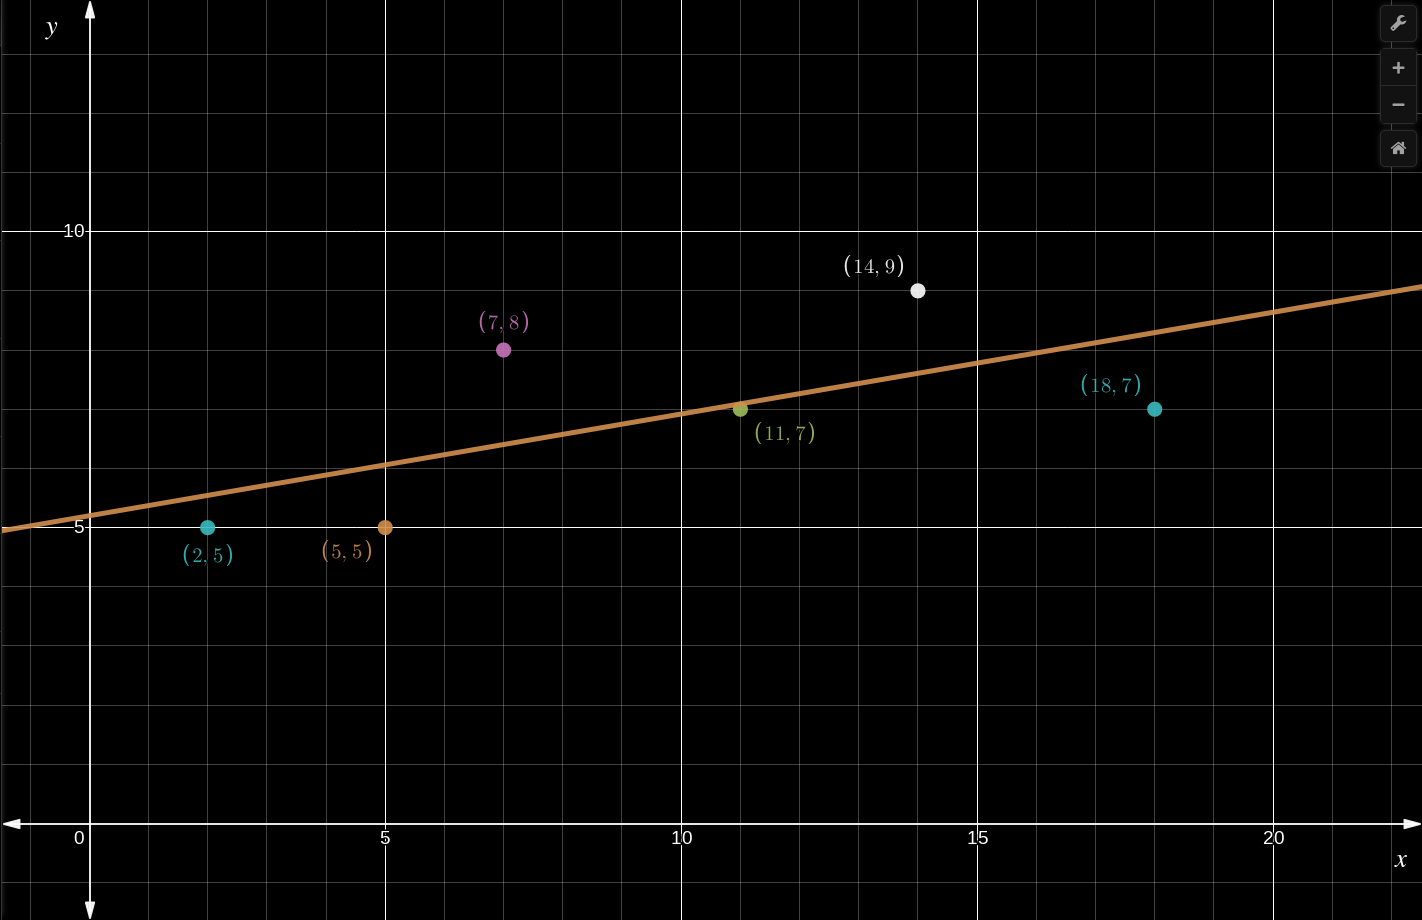
\includegraphics[width=8cm]{line}
}
% -------------------------------------------------------------------------
\frame[t] {
	\frametitle{Least squares}
	\framesubtitle{Recapitulation}

	You have a bunch of data points and suspect that a polynomial function $y=Ax+B$ from this points is a good model.

	You build a matrix $A$ and a vector $b$ from the polynomial and the points.

	The polynomial coefficients are a vector $x$ so $Ax=b$

	Then $x=(A^\intercal A)^{-1}A^\intercal b$


}
% -------------------------------------------------------------------------
\frame[t] {
	\frametitle{Least squares}
	\framesubtitle{Don't worry, its XXI century}

	So the key is calculate $x=(A^\intercal A)^{-1}A^\intercal b$.

	But you don't need to do this by hand like Gauss did.

	See the code, in this case Javascript code, using the mathjs package.


}
% -------------------------------------------------------------------------
\begin{frame}[fragile]
	\begin{lstlisting}
const { multiply, transpose, inv, matrix, format } = require( "mathjs")

const solve = (A, b) => {
	const transposed    = transpose(A)
	const product       = multiply(transposed, A)
	const inverse       = inv(product)
	const pseudoInverse = multiply(inverse,transposed)
	const x             = multiply(pseudoInverse, b)
	return x
}

const A = matrix([[2,1],[5,1],[7,1],[11,1],[14,1],[18,1]])
const b = matrix([5,5,8,7,9,7])

console.log(format(solve(A, b),5))
\end{lstlisting}
\end{frame}
% -------------------------------------------------------------------------
\begin{frame}[fragile,t]
	\frametitle{Least squares}
	\framesubtitle{The polynomial function}
	Get a terminal and do the magic
\end{frame}
% -------------------------------------------------------------------------
\begin{frame}[fragile,t]
	\frametitle{Least squares}
	\framesubtitle{The polynomial function}
	Get a terminal and do the magic
	\begin{lstlisting}
		$ node ls.js
		[0.17183, 5.2009]
	\end{lstlisting}
\end{frame}

% -------------------------------------------------------------------------
\frame[t] {
	\frametitle{Least squares}
	\framesubtitle{Going further}
	Mind blowing is coming

	To avert catastrophic damage in our brains it's time to rename things

	In the example we found a line $y=mx+b$, now:

	$m$ becomes $a_1$

	$b$ becomes $a_0$

	$x$ becomes $x_1$

	$y$ remains the same

	The found line, then, becomes

	$$
		y=a_1x_1+a_0=0.17183x_1+5.2009
	$$

	\textbf{Nothing has changed}, only the names.
}
% -------------------------------------------------------------------------
\frame[t] {
	\frametitle{Least squares}
	\framesubtitle{The polynomial function}

	In the example we picked a line for regression.

	A line in a plane can be expressed as a polynomial function $P(x_1)$ where $y$ (the dependent variable, a real number) is a
	function of $x_1$ (the independent variable, a real number)
	$$
		y \colon \mathbb{R} \to \mathbb{R} = P(x_1) = a_1x_1 + a_0
	$$

	But there are others $P(x_1)$s, for example:

	$$
		y \colon \mathbb{R} \to \mathbb{R} = P(x_1) = a_2x_1^2 + a_1x_1 + a_0
	$$

	What about using that quadratic function as the model for the measured points?
	
	\bigskip

	Let's see...

}
% -------------------------------------------------------------------------
\frame[t] {
	\frametitle{Least squares}
	\framesubtitle{A curve as a model}

	That is the curve:
	$
		y = a_2x_1^2 + a_1x_1 + a_0
	$

	And those are the points:
	$(2,5),(5,5),(7,8),(11,7),(14,9),(18,7)$

	Replacing $x_1$ and $y$ in each point, and switching terms:
	$$
	a_2x_1^2 + a_1x_1 + a_0 = 5
	$$



}
% -------------------------------------------------------------------------
\end{document}